\section{ПРОЕКТНАЯ ЧАСТЬ}

\subsection{Общий подход к проектированию}

Целью проектной части является построение backend-архитектуры, которая покрывает основные сценарии взаимодействия тренера и спортсмена и при этом остаётся расширяемой. Система должна быть пригодна для развития: добавления новых видов спорта, подключения внешних клиентов, появления дополнительных аналитических модулей и интеграций со спортивными устройствами.

Для решения этой задачи выбран микросервисный подход. Он позволяет разделить систему на независимые компоненты по предметным областям. В CoachLink такими областями являются авторизация, профили и связи пользователей, тренировочный процесс, уведомления, аналитика и AI-рекомендации.

Монолитная архитектура для первой версии могла бы быть проще в реализации, однако она хуже демонстрирует независимость предметных модулей и сложнее масштабируется организационно. В системе «тренер-спортсмен» отдельные части имеют разную природу. Например, сервис авторизации отвечает за безопасность и токены, сервис тренировок --- за предметную логику назначений и отчётов, сервис уведомлений --- за реакцию на события, а сервис аналитики --- за расчёт показателей. Разделение этих частей повышает ясность архитектуры.

Проектирование выполнялось с учётом следующих принципов:

\begin{enumerate}
\def\labelenumi{\arabic{enumi}.}
\tightlist
\item
  единая точка входа для внешних клиентов;
\item
  разделение ответственности между сервисами;
\item
  собственная база данных для stateful-сервисов;
\item
  использование событий для асинхронных операций;
\item
  использование внутренних API для синхронных межсервисных запросов;
\item
  документирование публичного API;
\item
  возможность расширения предметной модели.
\end{enumerate}

\subsection{Высокоуровневая архитектура}

Внешний клиент взаимодействует с платформой через API Gateway. Клиентом может быть мобильное приложение, web-интерфейс или другой сервис. В рамках данной работы клиентская часть не рассматривается как результат разработки, а используется только как потребитель REST API.

API Gateway проверяет авторизацию и перенаправляет запросы к backend-сервисам. Сервисы реализованы на Go и взаимодействуют между собой через HTTP и NATS JetStream. Для хранения данных используется PostgreSQL. Для генерации AI-рекомендаций используется локальный LLM-сервер Ollama. На рисунке~\ref{fig:components-scheme} представлена компонентная схема backend-платформы.

\begin{figure}[H]
  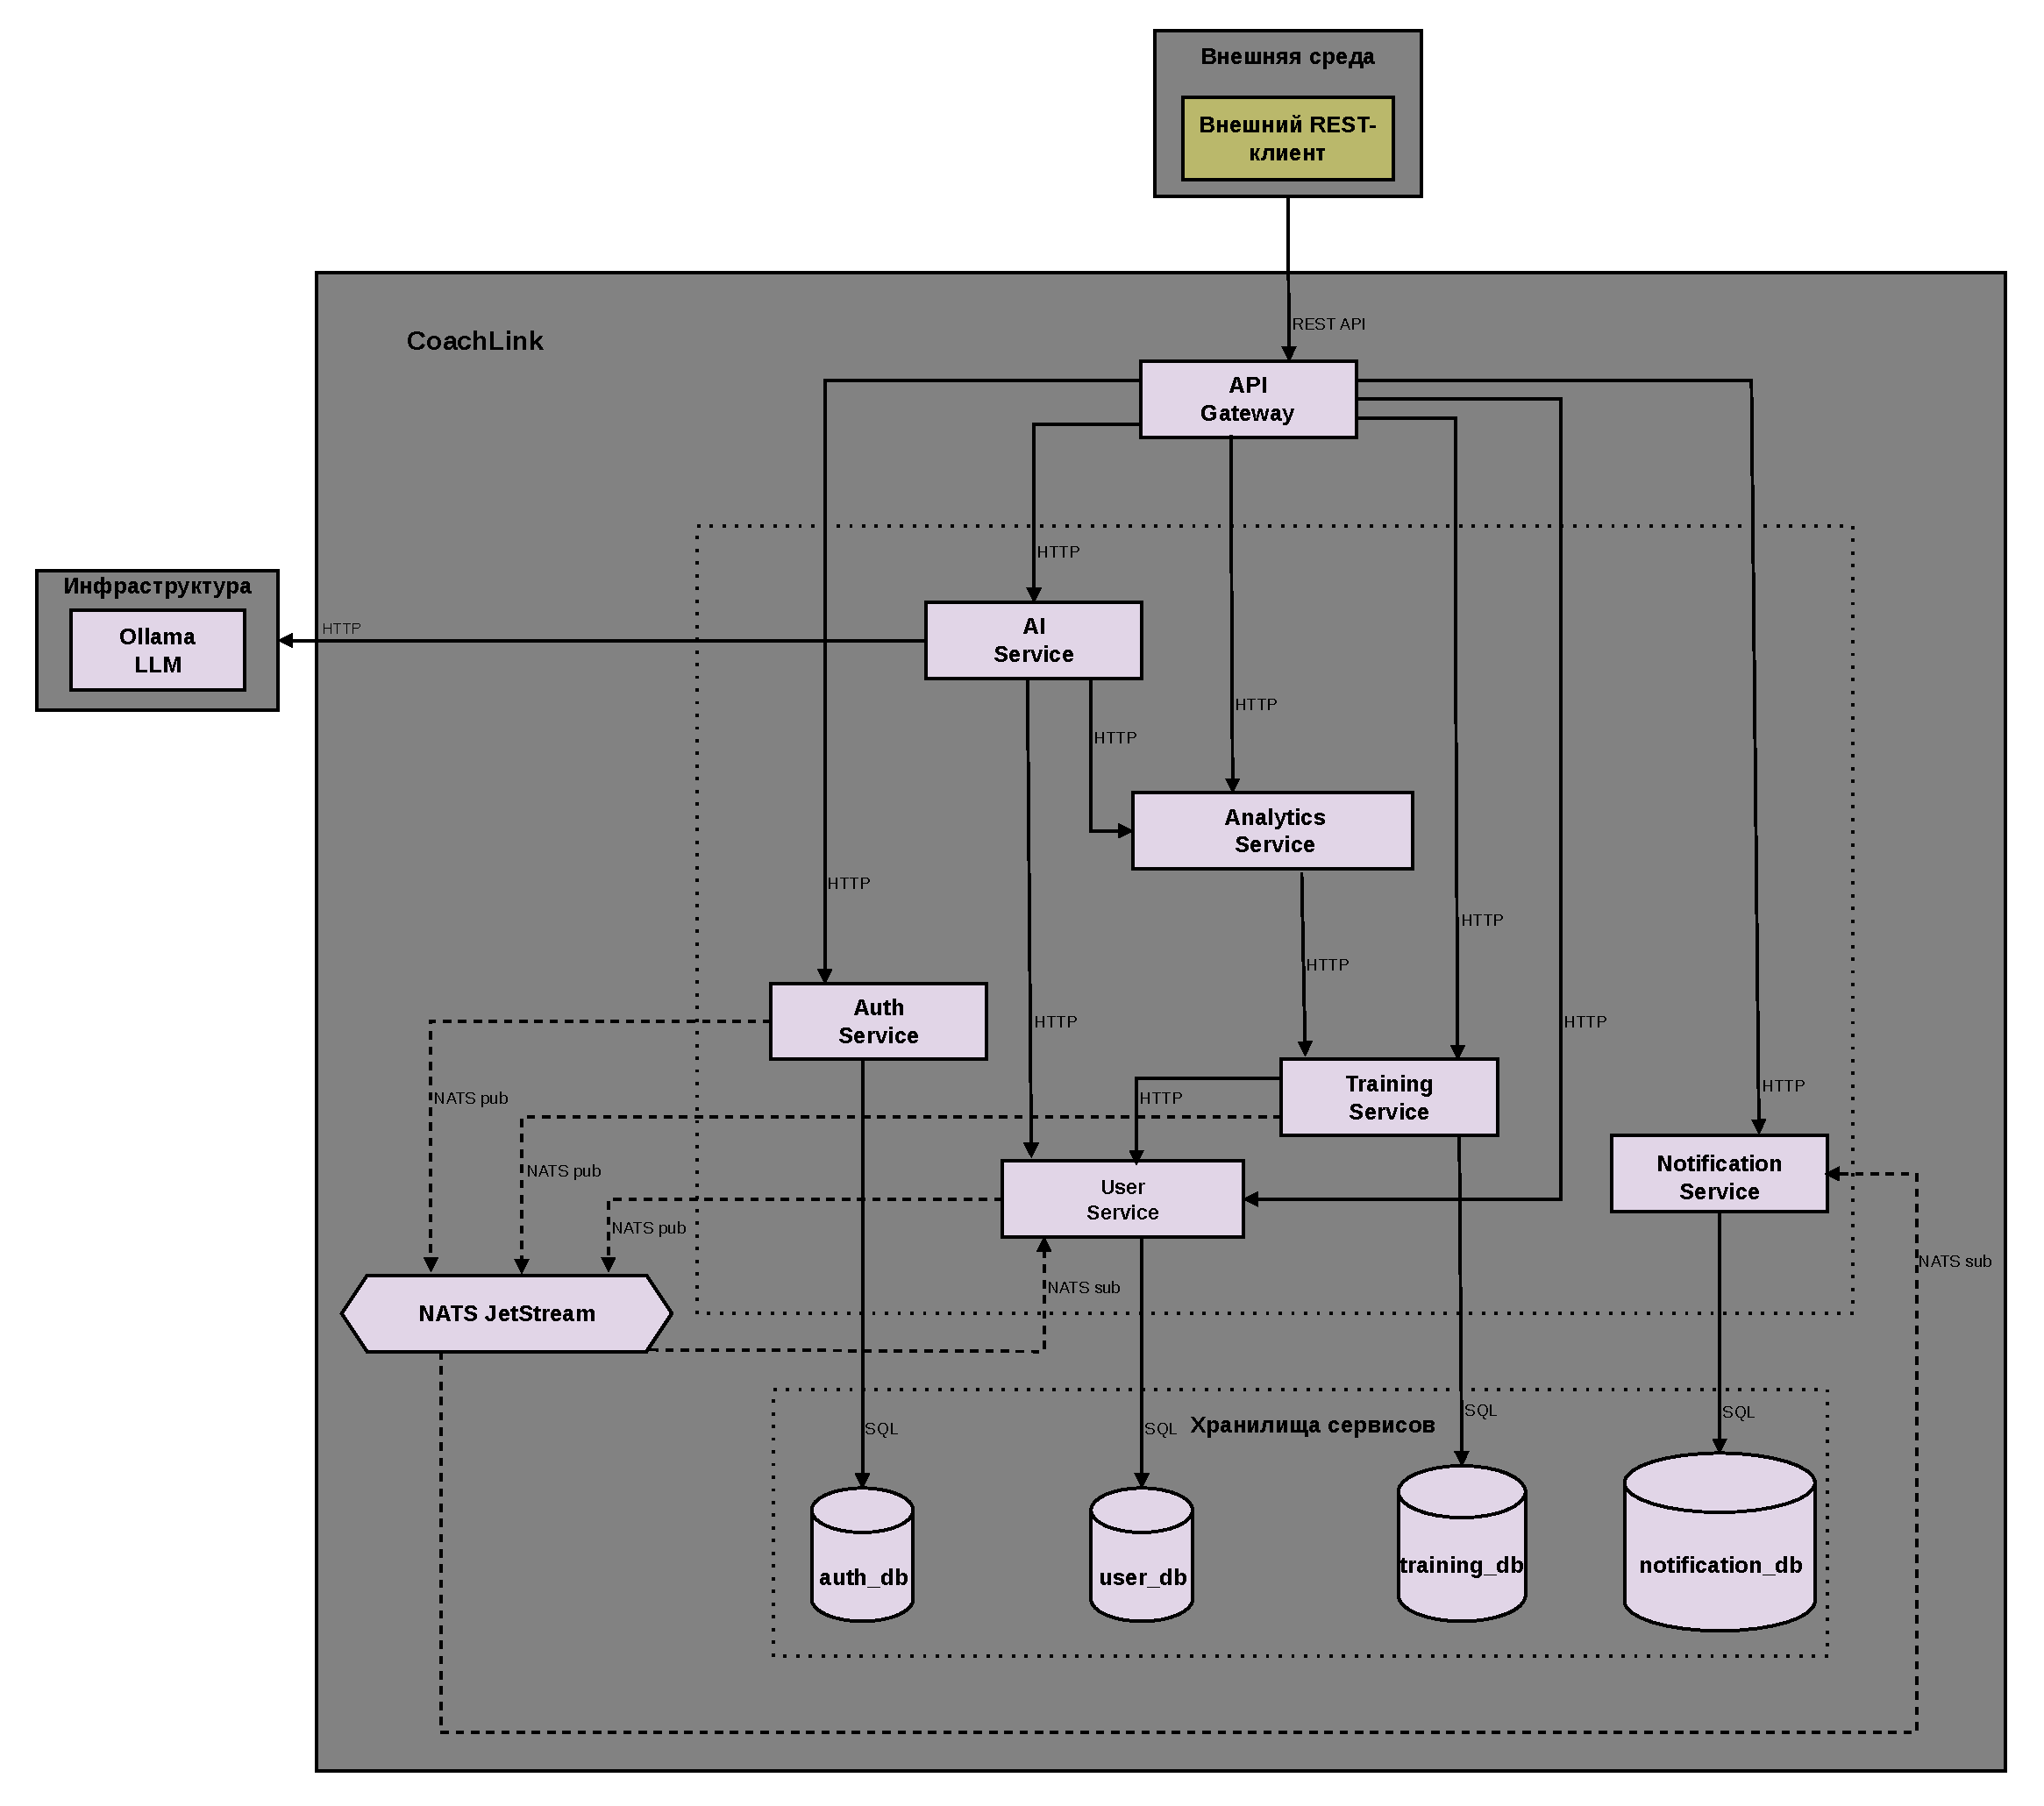
\includegraphics[page=1,width=\textwidth]{inc/components-sheme_cropped.pdf}
  \caption{Компонентная схема backend-платформы}
  \label{fig:components-scheme}
\end{figure}

В такой архитектуре API Gateway не содержит бизнес-логики. Его задача --- принять запрос, проверить JWT, добавить служебные заголовки и передать запрос в нужный сервис. Предметные правила остаются внутри соответствующих сервисов.

\subsection{Состав сервисов}

\subsubsection{API Gateway}

API Gateway является входной точкой для всех публичных HTTP-запросов. Он решает следующие задачи:

\begin{itemize}
\tightlist
\item
  маршрутизация запросов по префиксам;
\item
  проверка JWT access token;
\item
  извлечение идентификатора пользователя, роли и логина из токена;
\item
  проброс пользовательского контекста во внутренние сервисы через заголовки;
\item
  обработка CORS;
\item
  предоставление health-check endpoint.
\end{itemize}

Публичные маршруты без авторизации ограничены регистрацией, входом и обновлением токена:

\begin{itemize}
\tightlist
\item
  \passthrough{\lstinline!POST /api/v1/auth/register!};
\item
  \passthrough{\lstinline!POST /api/v1/auth/login!};
\item
  \passthrough{\lstinline!POST /api/v1/auth/refresh!}.
\end{itemize}

Остальные маршруты требуют заголовок \passthrough{\lstinline!Authorization: Bearer <token>!}. После успешной проверки Gateway устанавливает заголовки:

\begin{itemize}
\tightlist
\item
  \passthrough{\lstinline!X-User-ID!};
\item
  \passthrough{\lstinline!X-User-Role!};
\item
  \passthrough{\lstinline!X-User-Login!}.
\end{itemize}

Такой подход реализует паттерн API Gateway, описанный в работах по микросервисной архитектуре~\cite{richardson-microservices}: аутентификация выполняется один раз на входе, а внутренние сервисы доверяют Gateway и используют переданные заголовки для авторизации. Это исключает необходимость передавать JWT-секрет каждому сервису и упрощает добавление новых сервисов в систему.

\subsubsection{Auth Service}

Auth Service отвечает за учётные данные и токены. В его область ответственности входят:

\begin{itemize}
\tightlist
\item
  регистрация пользователя;
\item
  валидация логина, email, пароля и роли;
\item
  хеширование пароля;
\item
  вход пользователя;
\item
  выпуск access token и refresh token;
\item
  обновление пары токенов;
\item
  отзыв refresh token при logout;
\item
  публикация события регистрации.
\end{itemize}

Access token реализован как JWT. В payload токена включаются:

\begin{lstlisting}
{
  "sub": "uuid пользователя",
  "login": "user_login",
  "role": "coach | athlete",
  "exp": 1234567890,
  "iat": 1234567890
}
\end{lstlisting}

Refresh token хранится в базе данных не в открытом виде, а в виде SHA-256 хеша. Это снижает риск компрометации токена при утечке базы данных. При refresh старый токен удаляется, а пользователю выдаётся новая пара токенов.

После успешной регистрации Auth Service публикует событие \passthrough{\lstinline!coachlink.user.registered!}. Это событие используется User Service для создания пользовательского профиля.

\subsubsection{User Service}

User Service отвечает за доменную информацию о пользователях. Он не хранит пароли и не выпускает токены. Его задачи:

\begin{itemize}
\tightlist
\item
  хранение профилей пользователей;
\item
  синхронизация профилей из события регистрации;
\item
  поиск пользователей по ФИО и логину;
\item
  управление заявками спортсмена тренеру;
\item
  управление связями тренер-спортсмен;
\item
  управление тренировочными группами;
\item
  предоставление внутренних API для других сервисов.
\end{itemize}

Связь тренера и спортсмена создаётся через заявку. Это решение выбрано для явного контроля доступа: спортсмен не может автоматически прикрепиться к тренеру без подтверждения. Тренер видит входящие заявки и может принять или отклонить их.

Тренировочные группы принадлежат тренеру. Добавлять в группу можно только спортсменов, которые уже связаны с этим тренером. Это предотвращает ситуацию, когда тренер назначает тренировку спортсмену, не входящему в его область ответственности.

\subsubsection{Training Service}

Training Service реализует центральную предметную логику платформы. Он отвечает за:

\begin{itemize}
\tightlist
\item
  создание тренировочных планов;
\item
  назначение планов спортсменам;
\item
  назначение планов группе;
\item
  получение списка назначений;
\item
  фильтрацию назначений;
\item
  удаление и архивирование назначений;
\item
  отправку отчётов;
\item
  хранение шаблонов тренировок;
\item
  предоставление внутренних API для аналитики.
\end{itemize}

Тренировочный план и назначение спроектированы как отдельные сущности, связанные отношением <<один ко многим>>. План содержит название, описание и дату тренировки, а назначение связывает план с конкретным спортсменом и хранит индивидуальный статус выполнения. Такое разделение необходимо для групповых тренировок: тренер создаёт один план, а система формирует отдельное назначение для каждого участника группы. Денормализация ФИО и логина спортсмена в таблице назначений позволяет фильтровать и отображать списки без дополнительных запросов в User Service, что устраняет проблему N+1 запросов при получении списка назначений тренера.

Назначение имеет статус:

\begin{itemize}
\tightlist
\item
  \passthrough{\lstinline!assigned!} --- задание назначено и ожидает отчёта;
\item
  \passthrough{\lstinline!completed!} --- спортсмен отправил отчёт;
\item
  \passthrough{\lstinline!archived!} --- тренер перенёс выполненное задание в архив.
\end{itemize}

Просроченность не хранится как отдельное поле, а вычисляется при чтении. Это уменьшает риск рассинхронизации данных. Назначение считается просроченным, если оно находится в статусе \passthrough{\lstinline!assigned!}, а дата выполнения уже прошла.

\subsubsection{Notification Service}

Notification Service реализует паттерн событийного подписчика: он не вызывается напрямую другими сервисами, а подписывается на события NATS JetStream и реагирует на них созданием записей в таблице \passthrough{\lstinline!notifications!}. Для каждого типа события создаётся отдельный durable consumer, что обеспечивает независимую обработку и позволяет восстановить пропущенные сообщения после перезапуска сервиса.

Сервис обрабатывает следующие события:

\begin{itemize}
\tightlist
\item
  заявка спортсмена тренеру;
\item
  принятие или отклонение заявки;
\item
  назначение тренировки;
\item
  удаление задания;
\item
  отправка отчёта;
\item
  добавление спортсмена в группу;
\item
  удаление спортсмена из группы.
\end{itemize}

Пользователь может получить список уведомлений, отфильтровать их по признаку прочтения, получить количество непрочитанных уведомлений в ответе списка и отметить уведомления как прочитанные. Также сервис хранит FCM-токены устройств. Если Firebase credentials не настроены, push-доставка отключается, но уведомления продолжают сохраняться в базе данных.

\subsubsection{Analytics Service}

Analytics Service является stateless-сервисом. Он не имеет собственной базы данных, а получает данные из Training Service через внутренние API. Такое решение исключает проблему синхронизации аналитической базы с основной базой тренировок и гарантирует, что результаты агрегации всегда вычисляются по актуальным данным. При необходимости масштабирования аналитика может быть вынесена в отдельное хранилище без изменения публичного API.

Сервис предоставляет три основных представления данных:

\begin{itemize}
\tightlist
\item
  сводку по спортсмену;
\item
  прогресс по неделям или месяцам;
\item
  обзор по спортсменам тренера.
\end{itemize}

Каждое представление формируется из набора ключевых метрик тренировочного процесса:

\begin{itemize}
\tightlist
\item
  количество отчётов;
\item
  суммарная длительность;
\item
  средняя длительность;
\item
  суммарная дистанция;
\item
  средняя воспринимаемая нагрузка;
\item
  средний пульс;
\item
  максимальный пульс;
\item
  количество назначений;
\item
  процент выполнения.
\end{itemize}

\subsubsection{AI Service}

AI Service отвечает за генерацию рекомендаций по тренировочному процессу конкретного спортсмена на основе накопленных данных.

Публичный endpoint:

\begin{lstlisting}
POST /api/v1/ai/athletes/{id}/recommendations
\end{lstlisting}

Сервис доступен только тренеру. Перед генерацией он проверяет через User Service, что спортсмен действительно связан с текущим тренером. Затем AI Service получает из Analytics Service сводную статистику и последние отчёты спортсмена. Количество отчётов ограничено пятью, чтобы prompt оставался компактным. Типовой сценарий --- рекомендации по последним 3-5 тренировкам.

Генерация выполняется через Ollama. Prompt составляется на русском языке и содержит конкретные данные: объём тренировок, длительность, дистанцию, субъективную нагрузку, пульс и комментарии спортсмена. AI-модуль является вспомогательным инструментом и не заменяет решение тренера.

\subsection{Модель данных}

\subsubsection{Auth Service}

Auth Service использует две основные таблицы (таблица~\ref{tab:auth-db-tables}).

\begin{longtable}[]{|
  >{\raggedright\arraybackslash}p{(\columnwidth - 5\tabcolsep) * \real{0.4700}}|
  >{\raggedright\arraybackslash}p{(\columnwidth - 2\tabcolsep) * \real{0.4700}}|}
\caption{Таблицы Auth Service и их назначение}\label{tab:auth-db-tables}\\
\hline
\begin{minipage}[b]{\linewidth}\raggedright
Таблица
\end{minipage} & \begin{minipage}[b]{\linewidth}\raggedright
Назначение
\end{minipage} \\
\hline
\endhead
\hline
\endlastfoot
\passthrough{\lstinline!users!} & Учётные данные пользователя, роль и пароль в виде bcrypt-хеша \\ \hline
\passthrough{\lstinline!refresh\_tokens!} & Хеши refresh-токенов и срок их действия \\ \hline
\end{longtable}

Таблица \passthrough{\lstinline!users!} содержит логин, email, ФИО, роль, хеш пароля и временные метки. Роль ограничена значениями \passthrough{\lstinline!coach!} и \passthrough{\lstinline!athlete!} через CHECK-констрейнт, что исключает появление невалидных ролей на уровне базы данных. Логин имеет ограничение уникальности. Таблица \passthrough{\lstinline!refresh\_tokens!} связана с пользователем через внешний ключ с каскадным удалением: при удалении пользователя все его refresh-токены удаляются автоматически.

\subsubsection{User Service}

User Service использует следующие таблицы (таблица~\ref{tab:user-db-tables}).

\begin{longtable}[]{|
  >{\raggedright\arraybackslash}p{(\columnwidth - 2\tabcolsep) * \real{0.4700}}|
  >{\raggedright\arraybackslash}p{(\columnwidth - 2\tabcolsep) * \real{0.4700}}|}
\caption{Таблицы User Service и их назначение}\label{tab:user-db-tables}\\
\hline
\begin{minipage}[b]{\linewidth}\raggedright
Таблица
\end{minipage} & \begin{minipage}[b]{\linewidth}\raggedright
Назначение
\end{minipage} \\
\hline
\endhead
\hline
\endlastfoot
\passthrough{\lstinline!user\_profiles!} & Профили пользователей, синхронизированные из Auth Service \\ \hline
\passthrough{\lstinline!connection\_requests!} & Заявки спортсмена тренеру \\ \hline
\passthrough{\lstinline!coach\_athlete\_relations!} & Активные связи тренер-спортсмен \\ \hline
\passthrough{\lstinline!training\_groups!} & Тренировочные группы тренера \\ \hline
\passthrough{\lstinline!training\_group\_members!} & Состав тренировочных групп \\ \hline
\end{longtable}

Разделение \passthrough{\lstinline!users!} и \passthrough{\lstinline!user\_profiles!} отражает разделение ответственности сервисов: Auth Service хранит учётные данные, User Service --- доменную информацию для поиска, связей и групп. Таблица \passthrough{\lstinline!coach\_athlete\_relations!} использует UNIQUE-констрейнт на \passthrough{\lstinline!athlete\_id!}, что ограничивает спортсмена одним тренером и упрощает логику авторизации в Training Service и Analytics Service. Для текстового поиска по ФИО и логину используются trigram-индексы расширения \passthrough{\lstinline!pg\_trgm!}, обеспечивающие поиск подстрок и автодополнение.

\subsubsection{Training Service}

Training Service использует таблицы, описанные в таблице~\ref{tab:training-db-tables}.

\begin{longtable}{|>{\raggedright\arraybackslash}p{0.42\columnwidth}|>{\raggedright\arraybackslash}p{0.46\columnwidth}|}
\caption{Таблицы Training Service и их назначение}\label{tab:training-db-tables}\\
\hline
Таблица & Назначение \\
\hline
\endhead
\hline
\endlastfoot
\passthrough{\lstinline!training\_plans!} & Общая информация о тренировочном плане \\ \hline
\passthrough{\lstinline!training\_assignments!} & Назначение плана конкретному спортсмену \\ \hline
\passthrough{\lstinline!training\_reports!} & Отчёт спортсмена по назначению \\ \hline
\passthrough{\lstinline!training\_templates!} & Шаблоны тренировок тренера \\ \hline
\end{longtable}

Разделение плана и назначения на уровне таблиц соответствует проектному решению, описанному в разделе 2.3: один план порождает несколько назначений при групповой тренировке. Таблица \passthrough{\lstinline!training\_assignments!} содержит внешний ключ на план с каскадным удалением, CHECK-констрейнт на статус и денормализованные поля ФИО спортсмена. Отчёт связан с назначением через UNIQUE-ограничение: каждому назначению соответствует не более одного отчёта. Поле \passthrough{\lstinline!perceived\_effort!} ограничено диапазоном от 0 до 10 через CHECK-констрейнт.

\subsubsection{Notification Service}

Notification Service хранит данные в таблицах, представленных в таблице~\ref{tab:notification-db-tables}.

\begin{longtable}{|>{\raggedright\arraybackslash}p{0.42\columnwidth}|>{\raggedright\arraybackslash}p{0.46\columnwidth}|}
\caption{Таблицы Notification Service и их назначение}\label{tab:notification-db-tables}\\
\hline
Таблица & Назначение \\
\hline
\endhead
\hline
\endlastfoot
\passthrough{\lstinline!notifications!} & Уведомления пользователей \\ \hline
\passthrough{\lstinline!device\_tokens!} & FCM-токены устройств \\ \hline
\end{longtable}

В уведомлении хранится тип, заголовок, текст, дополнительные данные в JSONB, признак прочтения и дата создания. JSONB-поле позволяет добавлять к уведомлению контекст: идентификатор заявки, задания или группы.

\subsubsection{ER-диаграмма}

Общая структура данных представлена на ER-диаграмме (рисунок~\ref{fig:er-diagram}). Диаграмма отражает логические связи между основными сущностями платформы. В микросервисной архитектуре таблицы физически распределены по базам данных отдельных сервисов.

\begin{figure}[H]
  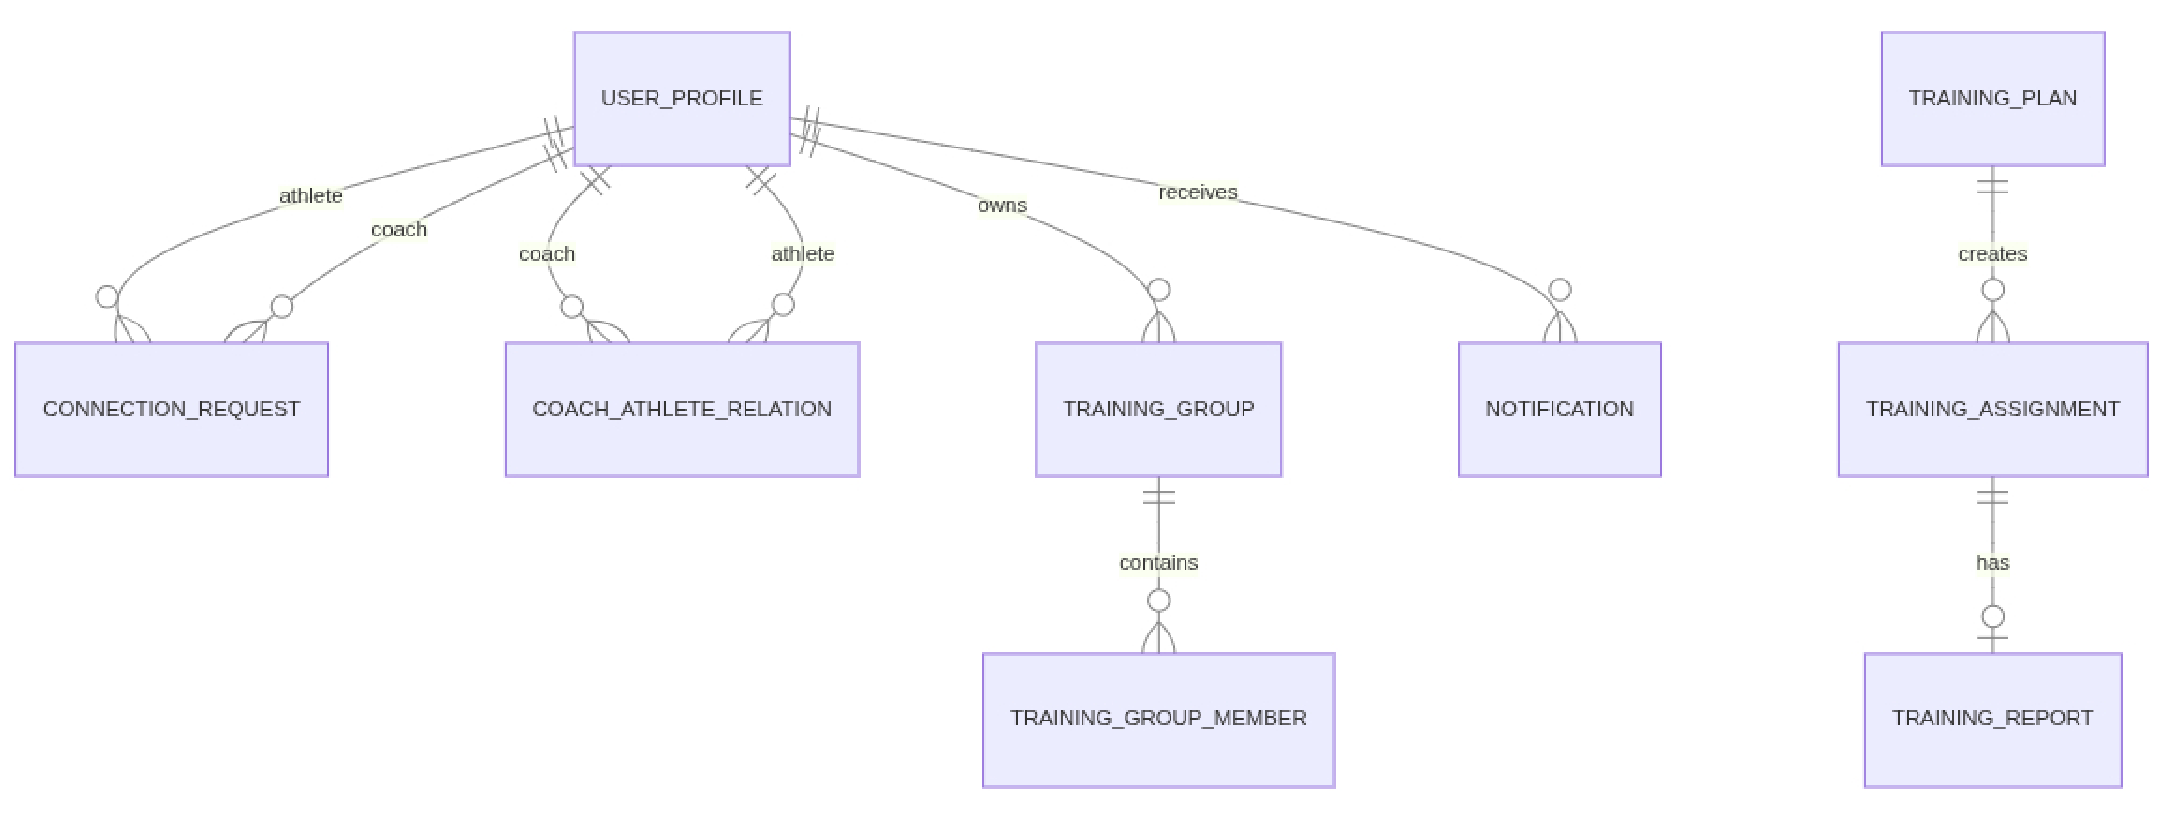
\includegraphics[page=1,width=\textwidth]{inc/ER-diagram_cropped.pdf}
  \caption{ER-диаграмма основных сущностей платформы CoachLink}
  \label{fig:er-diagram}
\end{figure}

\subsection{Межсервисное взаимодействие}

\subsubsection{Синхронное взаимодействие}

Синхронные HTTP-вызовы используются в случаях, когда результат нужен для выполнения текущего запроса.

Примеры:

\begin{enumerate}
\def\labelenumi{\arabic{enumi}.}
\tightlist
\item
  Training Service обращается к User Service при назначении плана группе, чтобы получить список участников группы;
\item
  Training Service получает профиль спортсмена, чтобы сохранить имя и логин в назначении;
\item
  Analytics Service обращается к Training Service за отчётами и агрегатами;
\item
  AI Service обращается к User Service для проверки связи тренера и спортсмена;
\item
  AI Service обращается к Analytics Service за сводкой и последними отчётами.
\end{enumerate}

Внутренние API не предназначены для внешних клиентов и доступны только сервисам внутри backend-платформы. При недоступности вызываемого сервиса вызывающий сервис возвращает клиенту ошибку с соответствующим HTTP-статусом. Повторные попытки для синхронных запросов не применяются, поскольку клиент ожидает ответ и повтор увеличил бы время ожидания. Для операций, допускающих задержку, используется асинхронное взаимодействие через NATS JetStream, где гарантия доставки обеспечивается брокером сообщений.

\subsubsection{Асинхронное взаимодействие}

Асинхронное взаимодействие реализовано через NATS JetStream. Оно используется там, где действие может быть выполнено после основного запроса и не должно блокировать пользователя.

Например, при создании тренировочного назначения Training Service публикует событие \passthrough{\lstinline!coachlink.training.assigned!}. Notification Service получает событие и создаёт уведомление для спортсмена. Если Notification Service временно недоступен, JetStream durable consumer позволяет обработать событие после восстановления сервиса.

В таблице~\ref{tab:nats-key-events} приведён список ключевых событий.

\begin{longtable}{|
  >{\raggedright\arraybackslash}p{0.34\columnwidth}|
  >{\raggedright\arraybackslash}p{0.16\columnwidth}|
  >{\raggedright\arraybackslash}p{0.18\columnwidth}|
  >{\raggedright\arraybackslash}p{0.20\columnwidth}|}
\caption{Ключевые события NATS JetStream в backend-платформе}\label{tab:nats-key-events}\\
\hline
Событие & Источник & Получатель & Назначение \\
\hline
\endfirsthead
\caption[]{Продолжение таблицы \thetable}\\
\hline
Событие & Источник & Получатель & Назначение \\
\hline
\endhead
\hline
\endlastfoot
\path|coachlink.user.registered| & Auth Service & User Service & Создание профиля \\ \hline
\path|coachlink.connection.requested| & User Service & Notification Service & Уведомление тренера \\ \hline
\path|coachlink.connection.accepted| & User Service & Notification Service & Уведомление спортсмена \\ \hline
\path|coachlink.connection.rejected| & User Service & Notification Service & Уведомление спортсмена \\ \hline
\path|coachlink.group.athlete_added| & User Service & Notification Service & Уведомление спортсмена \\ \hline
\path|coachlink.group.athlete_removed| & User Service & Notification Service & Уведомление спортсмена \\ \hline
\path|coachlink.training.assigned| & Training Service & Notification Service & Уведомление спортсмена \\ \hline
\path|coachlink.training.deleted| & Training Service & Notification Service & Уведомление спортсмена \\ \hline
\path|coachlink.report.submitted| & Training Service & Notification Service & Уведомление тренера \\ \hline
\end{longtable}

\subsection{Проектирование ключевых сценариев}

\subsubsection{Регистрация пользователя}

Сценарий регистрации включает несколько шагов: клиент отправляет запрос через API Gateway, Auth Service валидирует данные, хеширует пароль, создаёт пользователя и публикует событие в NATS JetStream, после чего User Service создаёт профиль. На рисунке~\ref{fig:registration-flow} показана последовательность взаимодействий при регистрации.

\begin{figure}[H]
  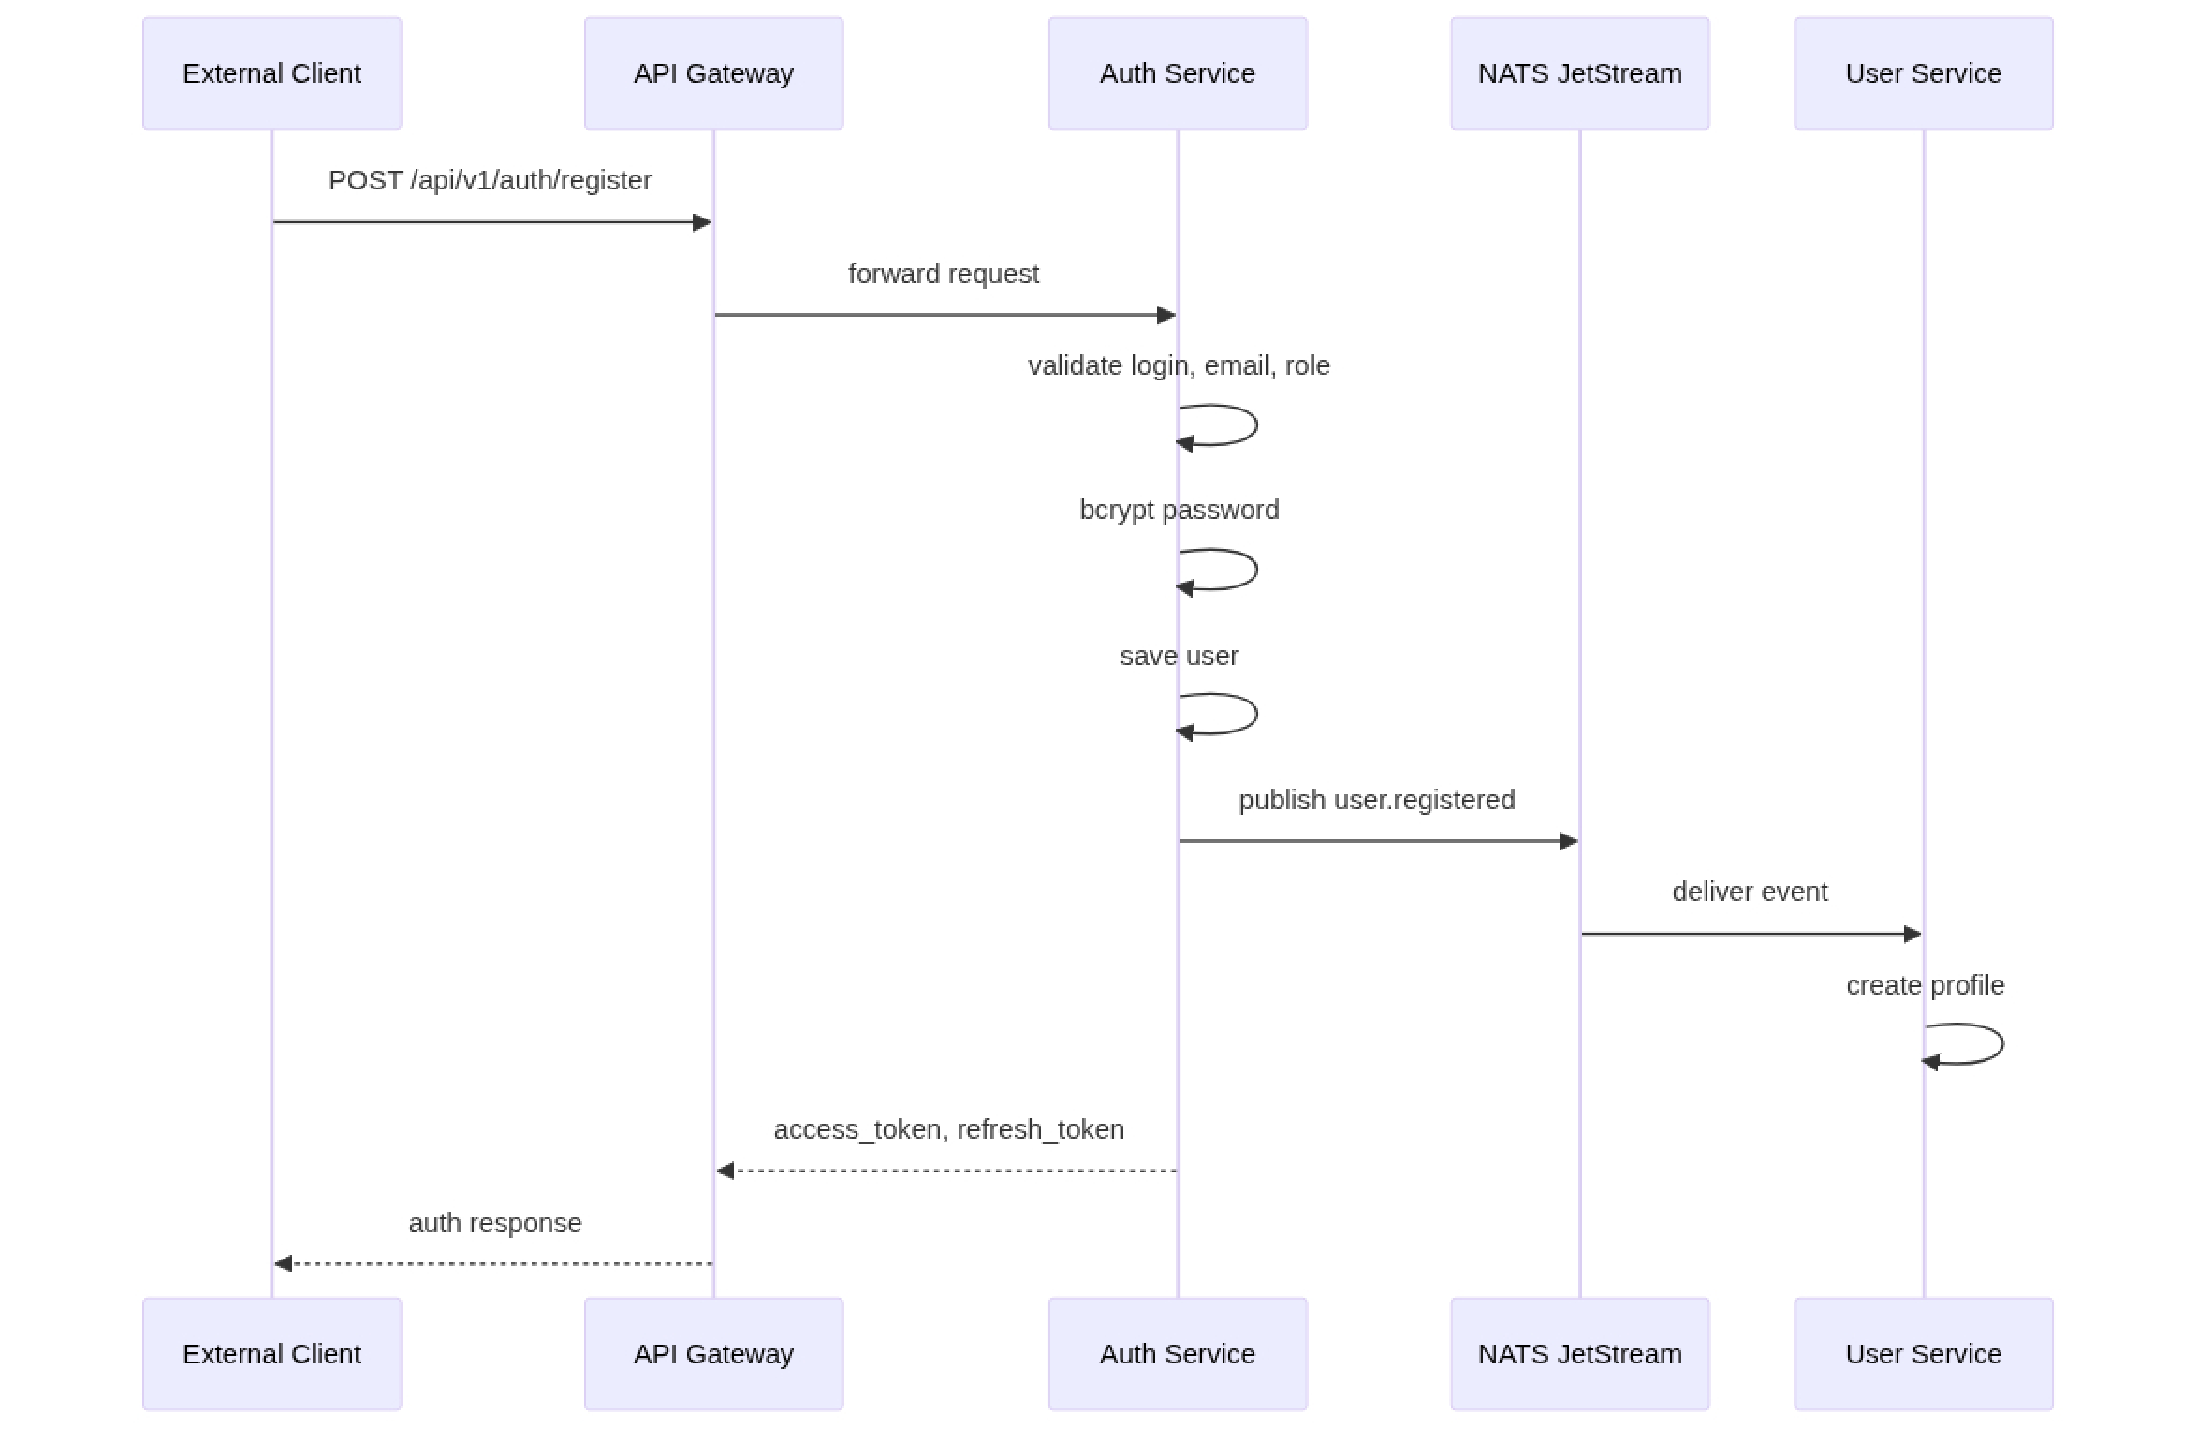
\includegraphics[page=1,width=\textwidth]{inc/user-registration_cropped.pdf}
  \caption{Последовательность взаимодействий при регистрации пользователя}
  \label{fig:registration-flow}
\end{figure}

\subsubsection{Создание связи тренер-спортсмен}

Для установления связи спортсмен отправляет заявку тренеру. Тренер получает уведомление и принимает или отклоняет заявку. При принятии создаётся запись в таблице связей. На рисунке~\ref{fig:coach-athlete-flow} представлена последовательность взаимодействий при создании связи.

\begin{figure}[H]
  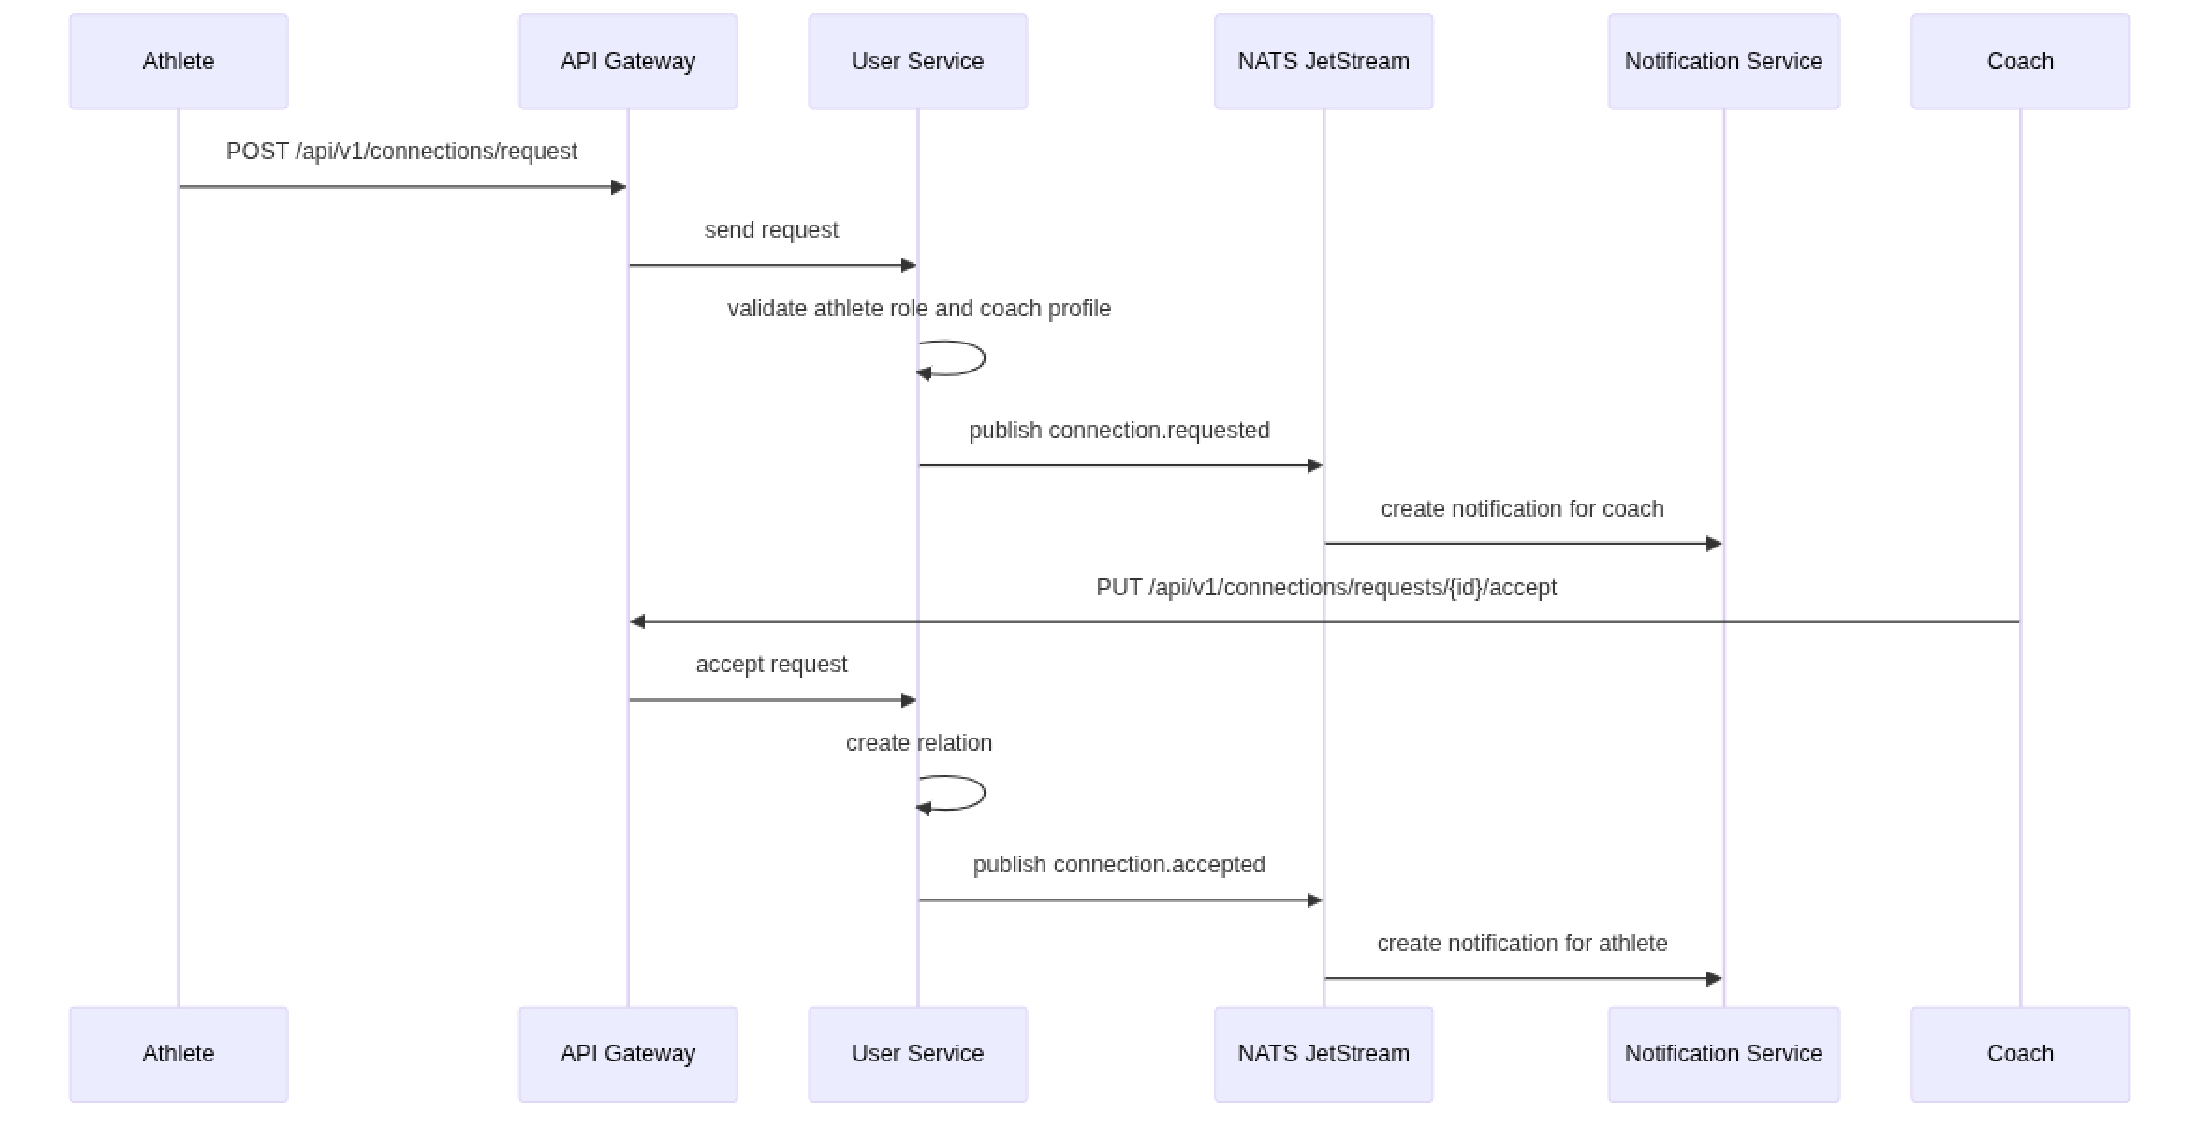
\includegraphics[page=1,width=\textwidth]{inc/user-coach_cropped.pdf}
  \caption{Последовательность взаимодействий при создании связи тренер-спортсмен}
  \label{fig:coach-athlete-flow}
\end{figure}

\subsubsection{Назначение тренировки группе}

При назначении тренировки группе Training Service обращается к User Service для получения списка участников, затем создаёт отдельное назначение для каждого спортсмена и публикует событие для Notification Service. На рисунке~\ref{fig:group-assignment-flow} показана последовательность взаимодействий при назначении тренировки группе.

\begin{figure}[H]
  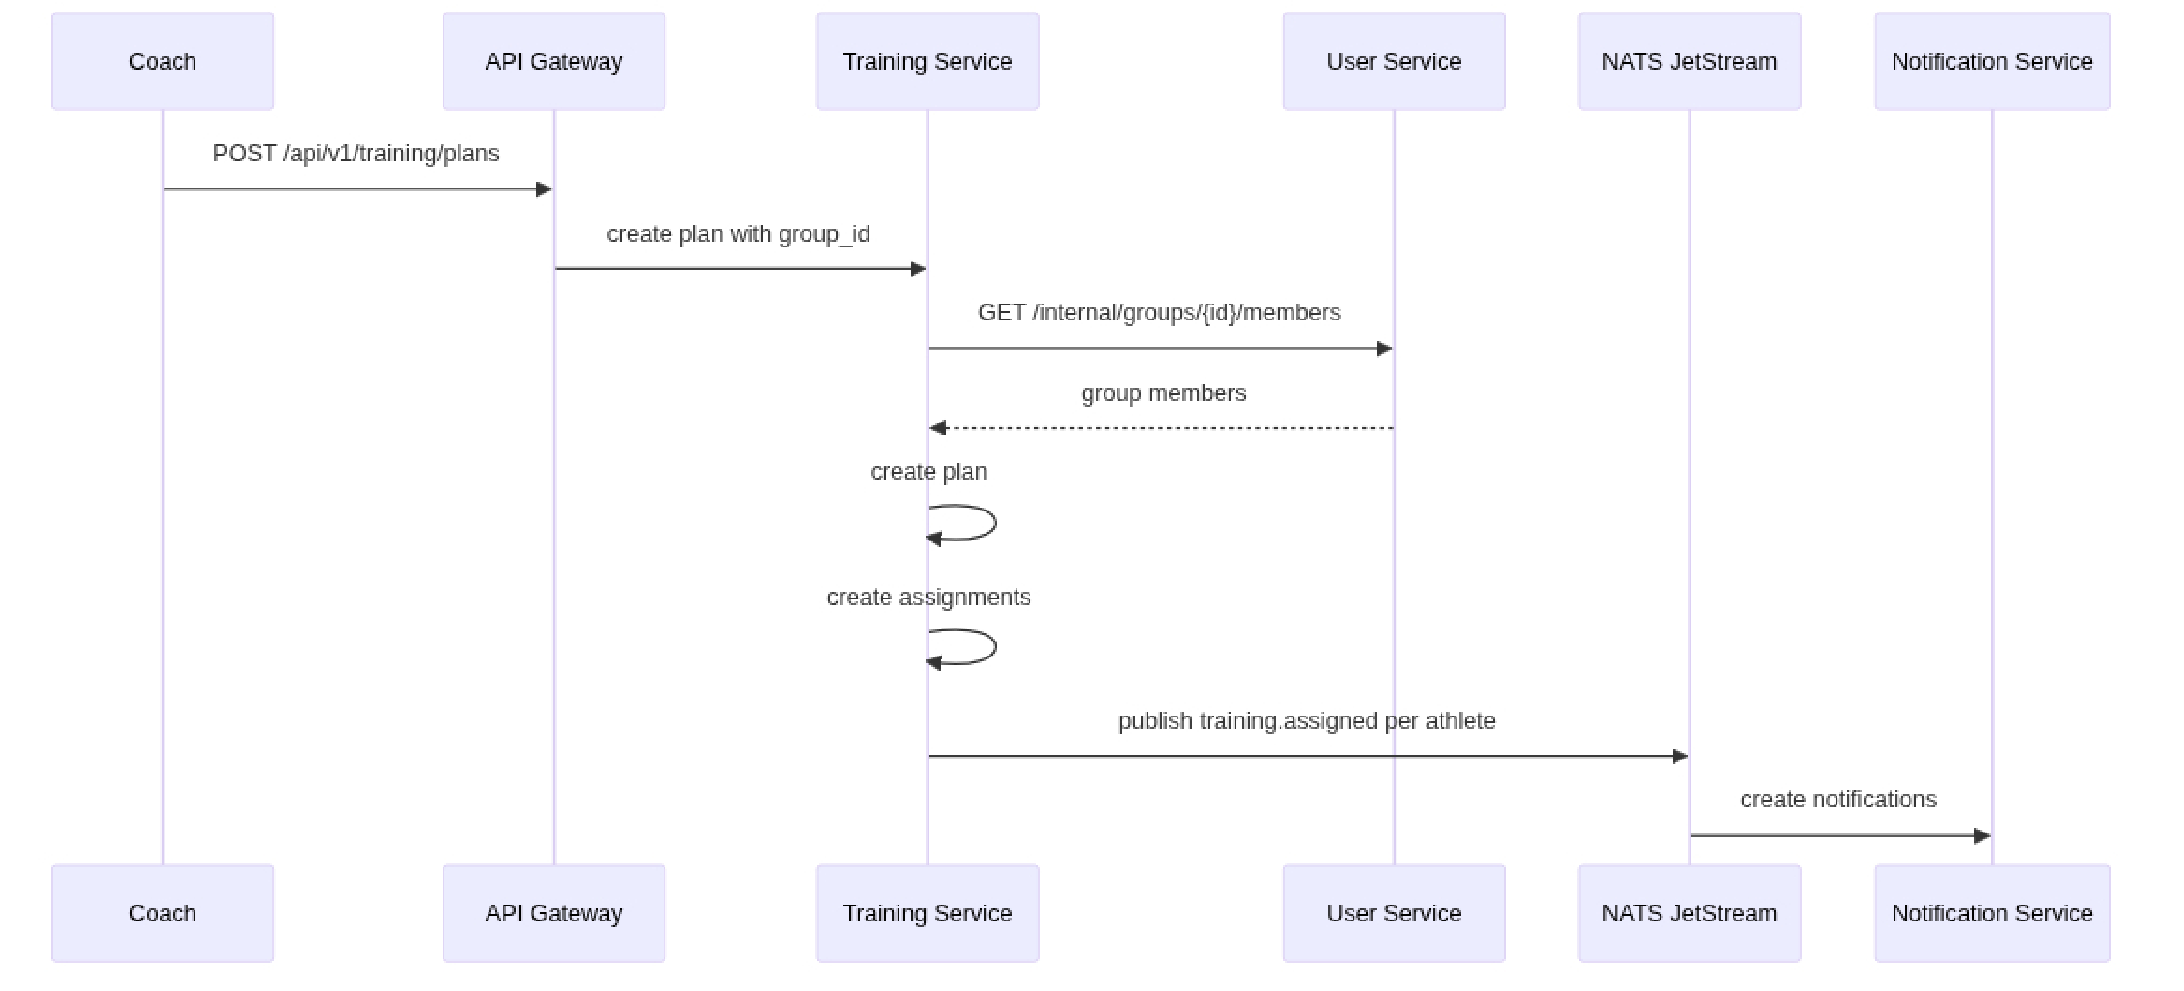
\includegraphics[page=1,width=\textwidth]{inc/trenirovka-grupe_cropped.pdf}
  \caption{Последовательность взаимодействий при назначении тренировки группе}
  \label{fig:group-assignment-flow}
\end{figure}

\subsubsection{Отправка отчёта}

При отправке отчёта спортсмен передаёт данные через API Gateway в Training Service. Сервис проверяет принадлежность назначения, сохраняет отчёт, меняет статус назначения и публикует событие, на которое реагирует Notification Service. На рисунке~\ref{fig:report-flow} показана последовательность взаимодействий при отправке отчёта.

\begin{figure}[H]
  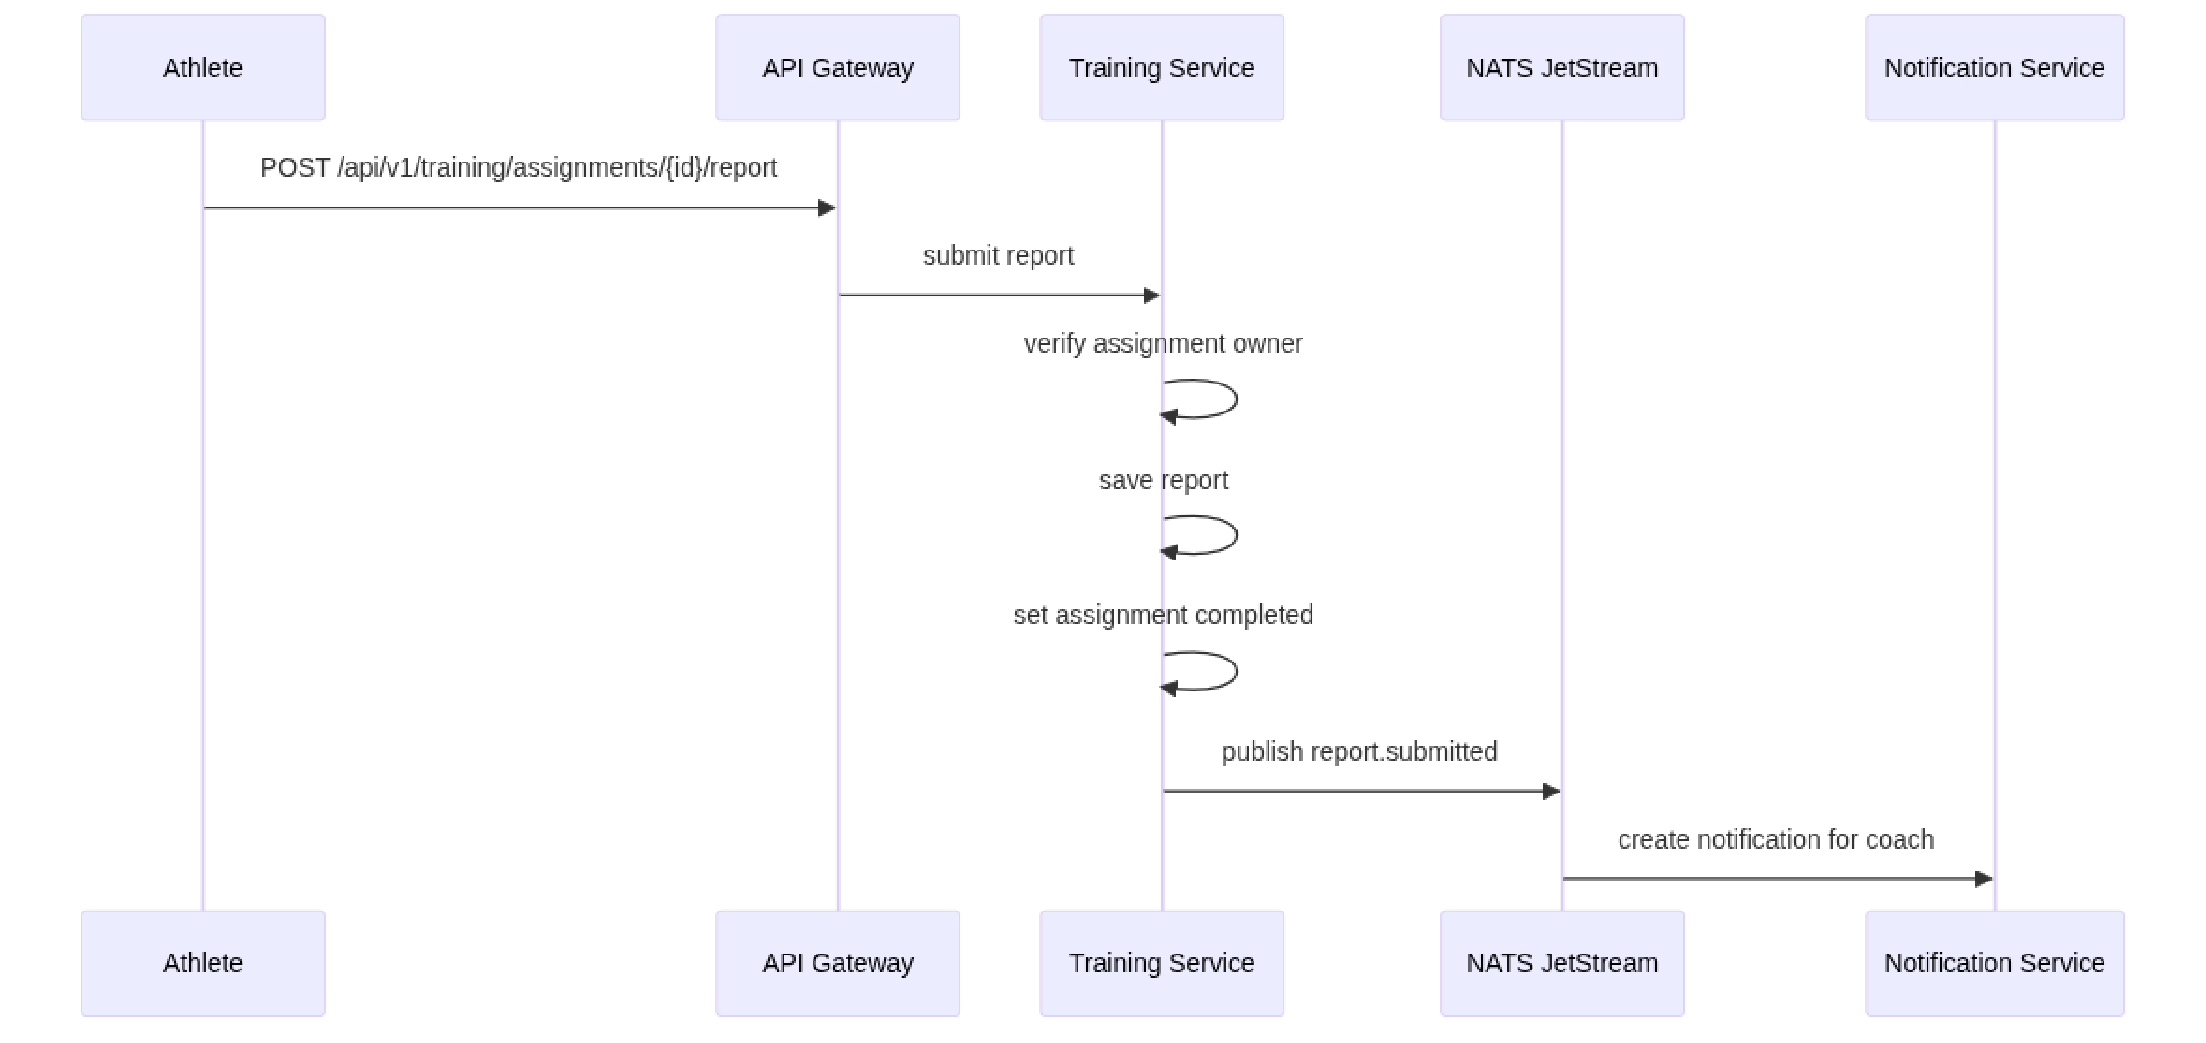
\includegraphics[page=1,width=\textwidth]{inc/report-sending_cropped.pdf}
  \caption{Последовательность взаимодействий при отправке отчёта}
  \label{fig:report-flow}
\end{figure}

\subsubsection{Получение AI-рекомендации}

Для получения AI-рекомендации тренер отправляет запрос через API Gateway в AI Service. Сервис проверяет связь тренера и спортсмена через User Service, получает статистику и последние отчёты из Analytics Service, формирует prompt и обращается к Ollama для генерации текста. На рисунке~\ref{fig:ai-recommendation-flow} показана последовательность взаимодействий при получении AI-рекомендации.

\begin{figure}[H]
  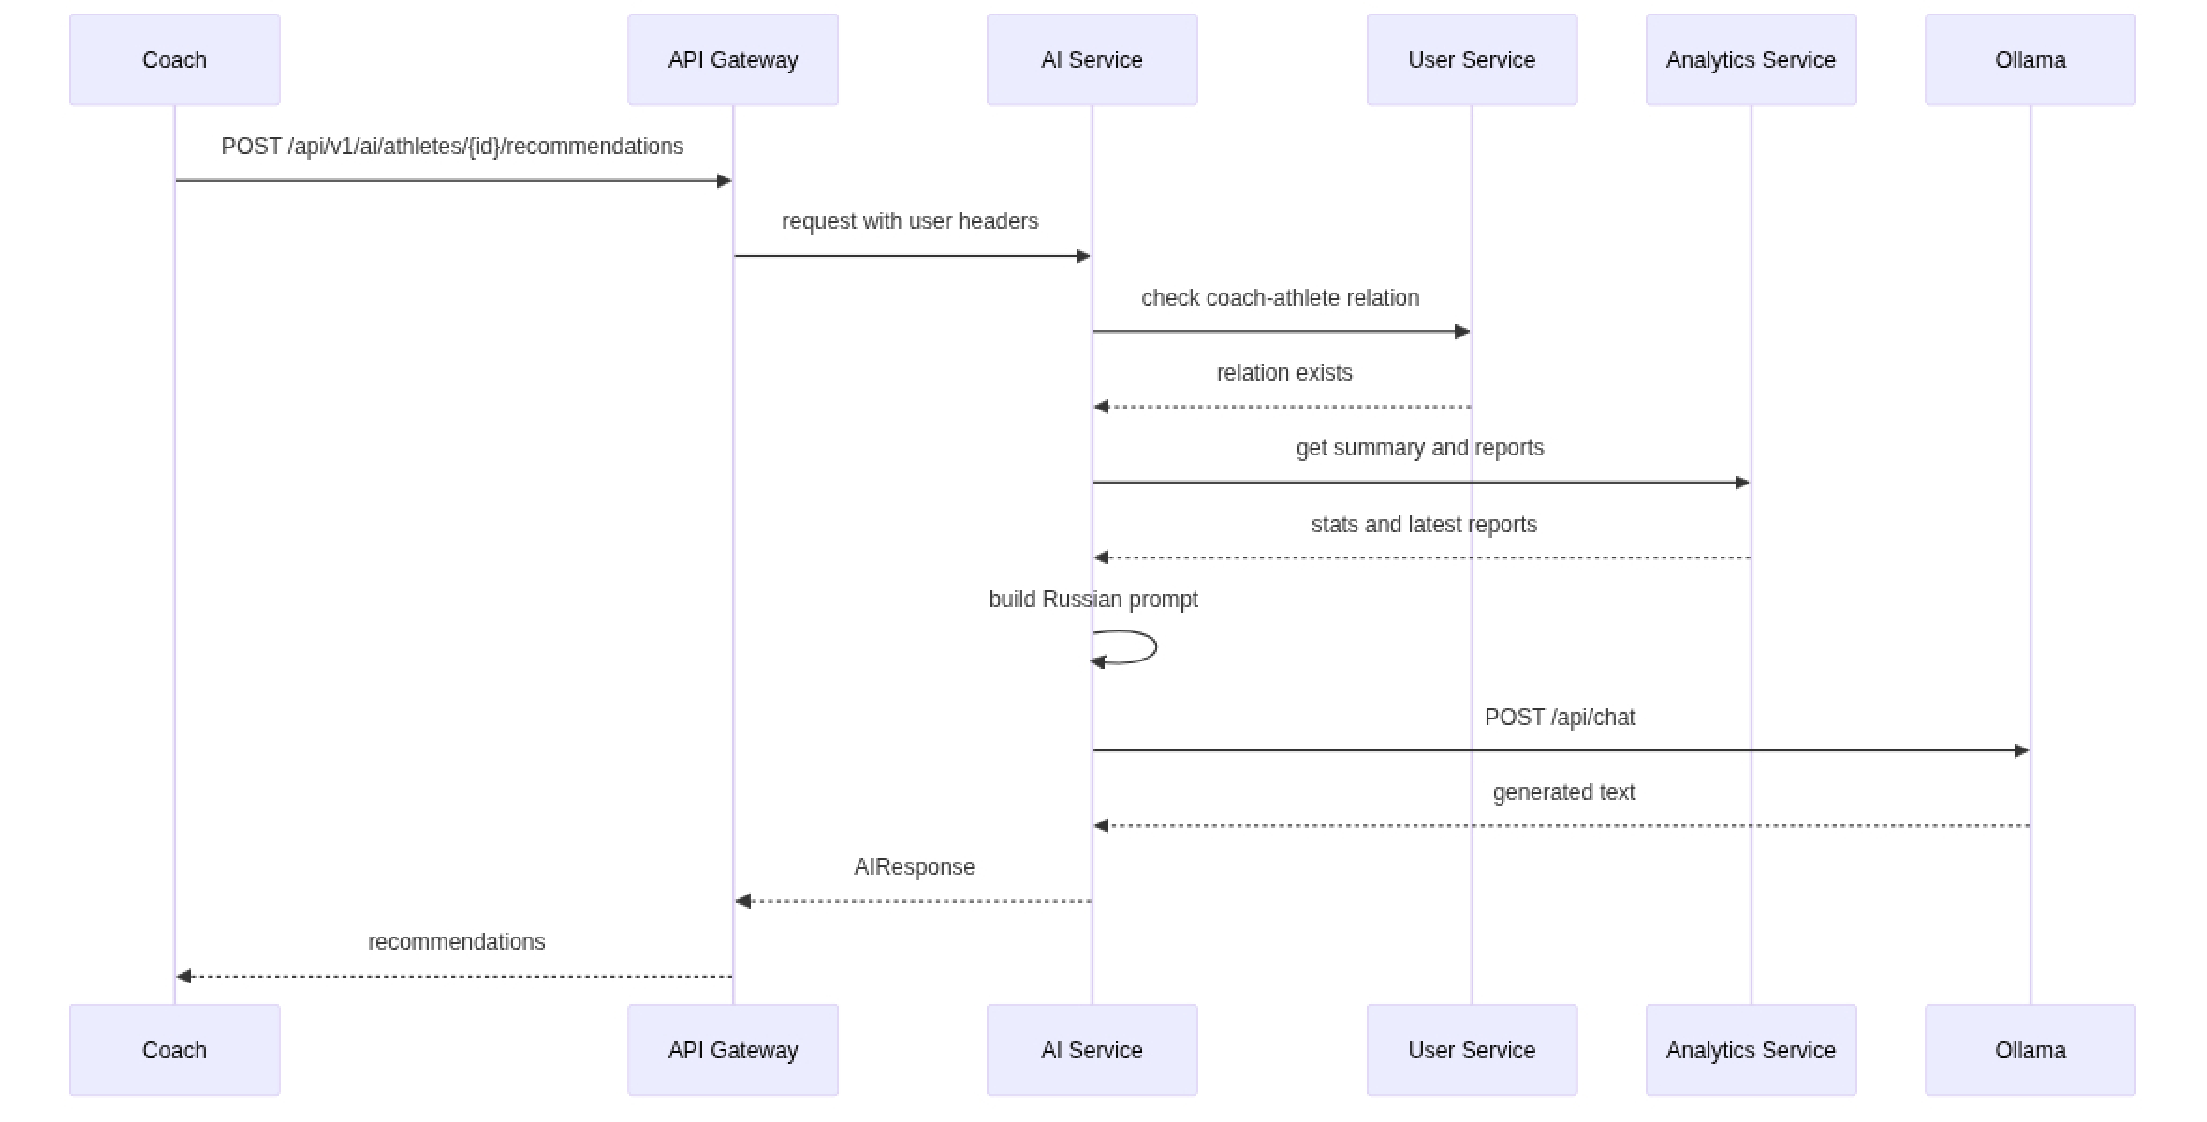
\includegraphics[page=1,width=\textwidth]{inc/AI-recomendation_cropped.pdf}
  \caption{Последовательность взаимодействий при получении AI-рекомендации}
  \label{fig:ai-recommendation-flow}
\end{figure}

\subsection{Проектирование публичного API}

Публичный API разделён на группы по предметным областям (таблица~\ref{tab:public-api-groups}).

\begin{longtable}{|>{\raggedright\arraybackslash}p{0.42\columnwidth}|>{\raggedright\arraybackslash}p{0.46\columnwidth}|}
\caption{Группы публичного API CoachLink}\label{tab:public-api-groups}\\
\hline
Группа & Назначение \\
\hline
\endfirsthead
\caption[]{Продолжение таблицы \thetable}\\
\hline
Группа & Назначение \\
\hline
\endhead
\hline
\endlastfoot
\passthrough{\lstinline!/api/v1/auth/*!} & Регистрация, вход, обновление и отзыв токенов \\ \hline
\passthrough{\lstinline!/api/v1/users/*!} & Профиль текущего пользователя и поиск \\ \hline
\passthrough{\lstinline!/api/v1/connections/*!} & Заявки и связи тренер-спортсмен \\ \hline
\passthrough{\lstinline!/api/v1/groups/*!} & Тренировочные группы \\ \hline
\passthrough{\lstinline!/api/v1/training/*!} & Планы, назначения, отчёты, шаблоны \\ \hline
\passthrough{\lstinline!/api/v1/notifications/*!} & Уведомления \\ \hline
\passthrough{\lstinline!/api/v1/analytics/*!} & Аналитика тренировок \\ \hline
\passthrough{\lstinline!/api/v1/ai/*!} & AI-рекомендации \\ \hline
\end{longtable}

Такое разделение упрощает маршрутизацию на уровне API Gateway и позволяет документировать каждую группу endpoint-ов независимо. При проектировании API соблюдались следующие принципы: версионирование через префикс \passthrough{\lstinline!/v1/!}, что позволяет вводить несовместимые изменения в будущих версиях без нарушения работы существующих клиентов; единообразный формат ошибок с HTTP-статусом и JSON-телом, содержащим описание ошибки; пагинация списков через query-параметры \passthrough{\lstinline!limit!} и \passthrough{\lstinline!offset!}; использование стандартных HTTP-методов в соответствии с семантикой REST. Полная спецификация API оформлена в формате OpenAPI и доступна в репозитории проекта.

\subsection{Расширяемость под другие виды спорта}

Хотя первая версия ориентирована на лёгкую атлетику, архитектура спроектирована с учётом расширения на другие виды спорта. Базовые сущности платформы --- пользователи, роли, связи, группы, назначения, уведомления и аналитические агрегаты --- не зависят от конкретного вида спорта и остаются неизменными при добавлении новых дисциплин.

Расширение предметной модели сосредоточено в Training Service. Конкретный механизм состоит в добавлении sport-specific полей в структуру тренировочного плана и отчёта. Например, для силовых видов спорта потребуются параметры подходов, повторений и веса, для плавания --- стиль и длина бассейна, для велоспорта --- средняя мощность и набор высоты. Эти поля могут быть реализованы через расширение схемы таблиц или через JSONB-поле с динамической структурой. При этом общий жизненный цикл назначения (создание, выполнение, отчёт, архивация), система уведомлений, аналитическая агрегация и API Gateway не требуют изменений.

\subsection{Выводы по главе 2}

В проектной части была предложена микросервисная backend-архитектура CoachLink. Архитектура включает API Gateway, сервис авторизации, сервис пользователей, сервис тренировок, сервис уведомлений, сервис аналитики и AI-сервис рекомендаций. Для хранения данных используется PostgreSQL, для событийного взаимодействия --- NATS JetStream, для локального развёртывания --- Docker Compose.

Спроектированная архитектура соответствует требованиям, сформулированным в аналитической главе. Она поддерживает ролевую модель, связи тренера и спортсмена, групповые назначения, стандартизированные отчёты, уведомления и аналитику. При этом система остаётся расширяемой: текущая реализация ориентирована на лёгкую атлетику, но базовая модель может быть адаптирована для других видов спорта.
